%This is a slight variation of the "sig-alternate.tex". We have added a
%\selfcite{myref} command to the sig-alternate.cls file and some explanations to
%the sig-alternate.tex file. Thus, sig-alternate.cls has been renamed to
%dads.cls and sig-alternate.tex has been renamed to dads[nn].tex

% This is "sig-alternate.tex" V1.9 April 2009
% This file should be compiled with V2.4 of "sig-alternate.cls" April 2009
%
% This example file demonstrates the use of the 'sig-alternate.cls'
% V2.4 LaTeX2e document class file. It is for those submitting
% articles to ACM Conference Proceedings WHO DO NOT WISH TO
% STRICTLY ADHERE TO THE SIGS (PUBS-BOARD-ENDORSED) STYLE.
% The 'sig-alternate.cls' file will produce a similar-looking,
% albeit, 'tighter' paper resulting in, invariably, fewer pages.
%
% ----------------------------------------------------------------------------------------------------------------
% This .tex file (and associated .cls V2.4) produces:
%       1) The Permission Statement
%       2) The Conference (location) Info information
%       3) The Copyright Line with ACM data
%       4) NO page numbers
%
% as against the acm_proc_article-sp.cls file which
% DOES NOT produce 1) thru' 3) above.
%
% Using 'sig-alternate.cls' you have control, however, from within
% the source .tex file, over both the CopyrightYear
% (defaulted to 200X) and the ACM Copyright Data
% (defaulted to X-XXXXX-XX-X/XX/XX).
% e.g.
% \CopyrightYear{2007} will cause 2007 to appear in the copyright line.
% \crdata{0-12345-67-8/90/12} will cause 0-12345-67-8/90/12 to appear in the copyright line.
%
% ---------------------------------------------------------------------------------------------------------------
% This .tex source is an example which *does* use
% the .bib file (from which the .bbl file % is produced).
% REMEMBER HOWEVER: After having produced the .bbl file,
% and prior to final submission, you *NEED* to 'insert'
% your .bbl file into your source .tex file so as to provide
% ONE 'self-contained' source file.
%
% ================= IF YOU HAVE QUESTIONS =======================
% Questions regarding the SIGS styles, SIGS policies and
% procedures, Conferences etc. should be sent to
% Adrienne Griscti (griscti@acm.org)
%
% Technical questions _only_ to
% Gerald Murray (murray@hq.acm.org)
% ===============================================================
%
% For tracking purposes - this is V1.9 - April 2009

\documentclass{dads}   %Changed for DADS
\usepackage{format}
\usepackage{macros}
\usepackage{macros_stm}
\usepackage{paper}
\usepackage{url}
\usepackage[colorlinks=true,linkcolor=blue,urlcolor=blue,citecolor=blue]{hyperref}
\begin{document}
\newboolean{showcomments}
\setboolean{showcomments}{true}
\ifthenelse{\boolean{showcomments}}
{ \newcommand{\mynote}[3]{
   \fbox{\bfseries\sffamily\scriptsize#1}
   {\small$\blacktriangleright$\textsf{\emph{\color{#3}{#2}}}$\blacktriangleleft$}}}
{ \newcommand{\mynote}[3]{}}
% One command per author:
\newcommand{\pf}[1]{\mynote{Pierre}{#1}{red}}
\newcommand{\hm}[1]{\mynote{Patrick}{#1}{pink}}
\newcommand{\vs}[1]{\mynote{Valerio}{#1}{blue}}
% --- Author Metadata here ---
\conferenceinfo{SAC'18}{April 9--13, 2018, Pau, France}
\CopyrightYear{2018} % Allows default copyright year (200x) to be over-ridden - IF NEED BE.
%\crdata{0-12345-67-8/90/01}  % Allows default copyright data (0-89791-88-6/97/05) to be over-ridden - IF NEED BE.
% --- End of Author Metadata ---

\title{A Locality-Aware Software Transactional Memory}

%\subtitle{[Slightly extended for DADS]
%\titlenote{A full version of this paper is available as
%\textit{Author's Guide to Preparing ACM SIG Proceedings Using
%\LaTeX$2_\epsilon$\ and BibTeX} at
%\texttt{www.acm.org/eaddress.htm}}}
%
% You need the command \numberofauthors to handle the 'placement
% and alignment' of the authors beneath the title.
%
% For aesthetic reasons, we recommend 'three authors at a time'
% i.e. three 'name/affiliation blocks' be placed beneath the title.
%
% NOTE: You are NOT restricted in how many 'rows' of
% "name/affiliations" may appear. We just ask that you restrict
% the number of 'columns' to three.
%
% Because of the available 'opening page real-estate'
% we ask you to refrain from putting more than six authors
% (two rows with three columns) beneath the article title.
% More than six makes the first-page appear very cluttered indeed.
%
% Use the \alignauthor commands to handle the names
% and affiliations for an 'aesthetic maximum' of six authors.
% Add names, affiliations, addresses for
% the seventh etc. author(s) as the argument for the
% \additionalauthors command.
% These 'additional authors' will be output/set for you
% without further effort on your part as the last section in
% the body of your article BEFORE References or any Appendices.

\numberofauthors{1} %  in this sample file, there are a *total*
% of EIGHT authors. SIX appear on the 'first-page' (for formatting
% reasons) and the remaining two appear in the \additionalauthors section.
%
\author{
% You can go ahead and credit any number of authors here,
% e.g. one 'row of three' or two rows (consisting of one row of three
% and a second row of one, two or three).
%
% The command \alignauthor (no curly braces needed) should
% precede each author name, affiliation/snail-mail address and
% e-mail address. Additionally, tag each line of
% affiliation/address with \affaddr, and tag the
% e-mail address with \email.
%
\alignauthor
No author info because of double-blind review.
% 1st. author
%\alignauthor
%Ben Trovato\titlenote{Dr.~Trovato insisted his name be first.}\\
%       \affaddr{Institute for Clarity in Documentation}\\
%       \affaddr{1932 Wallamaloo Lane}\\
%       \affaddr{Wallamaloo, New Zealand}\\
%       \email{trovato@corporation.com}
%% 2nd. author
%\alignauthor
%G.K.M. Tobin\titlenote{The secretary disavows
%any knowledge of this author's actions.}\\
%       \affaddr{Institute for Clarity in Documentation}\\
%       \affaddr{P.O. Box 1212}\\
%       \affaddr{Dublin, Ohio 43017-6221}\\
%       \email{webmaster@marysville-ohio.com}
%% 3rd. author
%\alignauthor Lars Th{\o}rv{\"a}ld\titlenote{This author is the
%one who did all the really hard work.}\\
%       \affaddr{The Th{\o}rv{\"a}ld Group}\\
%       \affaddr{1 Th{\o}rv{\"a}ld Circle}\\
%       \affaddr{Hekla, Iceland}\\
%       \email{larst@affiliation.org}
%\and  % use '\and' if you need 'another row' of author names
%% 4th. author
%\alignauthor Lawrence P. Leipuner\\
%       \affaddr{Brookhaven Laboratories}\\
%       \affaddr{Brookhaven National Lab}\\
%       \affaddr{P.O. Box 5000}\\
%       \email{lleipuner@researchlabs.org}
%% 5th. author
%\alignauthor Sean Fogarty\\
%       \affaddr{NASA Ames Research Center}\\
%       \affaddr{Moffett Field}\\
%       \affaddr{California 94035}\\
%       \email{fogartys@amesres.org}
%% 6th. author
%\alignauthor Charles Palmer\\
%       \affaddr{Palmer Research Laboratories}\\
%       \affaddr{8600 Datapoint Drive}\\
%       \affaddr{San Antonio, Texas 78229}\\
%       \email{cpalmer@prl.com}
}
%% There's nothing stopping you putting the seventh, eighth, etc.
%% author on the opening page (as the 'third row') but we ask,
%% for aesthetic reasons that you place these 'additional authors'
%% in the \additional authors block, viz.
%\additionalauthors{Additional authors: John Smith (The Th{\o}rv{\"a}ld Group,
%email: {\texttt{jsmith@affiliation.org}}) and Julius P.~Kumquat
%(The Kumquat Consortium, email: {\texttt{jpkumquat@consortium.net}}).}
\date{}
% Just remember to make sure that the TOTAL number of authors
% is the number that will appear on the first page PLUS the
% number that will appear in the \additionalauthors section.

\maketitle
\begin{abstract}
  Software transactional memory (STM) guarantees that a sequence of operations encapsulated into a transaction is executed atomically.
  This simple yet powerful paradigm is a promising direction for writing concurrent applications.
  %
  Recent STM designs employ a time-based approach to leverage the performance advantage of invisible reads.
  With the advent of many-core architectures and non-uniform memory architecture (NUMA), this design is however hitting the synchronization wall of the cache coherency protocols.
  %
  In this paper, we propose a novel and flexible approach to address this limitation.
  Our idea is to leverage the parallelism and the locality of applicative workloads to execute few global operations.
  To this end, we introduce a new STM design that supports invisible reads, lazy snapshots and can be tailored to be either disjoint access parallel, or NUMA-aware.
  Our empirical evaluation demonstrate that our design is sound.
\end{abstract}

% A category with the (minimum) three required fields
\category{H.4}{Information Systems Applications}{Miscellaneous}
%A category including the fourth, optional field follows...
\category{D.2.8}{Software Engineering}{Metrics}[complexity measures, performance measures]

\terms{Locality, Software Transactional Memory, NUMA}

\keywords{NUMA, STM}


\section{Introduction}
\labsection{introduction}

% why TM
The advent of chip level multiprocessing in commodity hardware has pushed applications to be more and more parallel in order to leverage the increase of computational power.
However, the art of concurrent programming is known to be a difficult task~\cite{Lee:2006:PT:1137232.1137289}, and new paradigms are required to help the programmer.
Among those paradigms, transactional memory (TM) is widely considered as a promising direction, in particular thanks to its simplicity~\cite{Dragojevic:2011:WSM:1924421.1924440}.

% the case for invisible optimistic reads and DAP
The engine that orchestrates concurrent transactions run by the application, i.e., the concurrency manager, is one of the core aspects of a STM implementation.
A large number of concurrency manager implementations exists, ranging from pessimistic lock-based implementations\vs{ref?} to completely optimistic ones\vs{ref?}, with~\cite{perelman2011smv} or without multi-version support\vs{ref?}.
Because application workloads exhibit in general a high degree of parallelism\vs{is this a known fact? for which applications? a ref that assess this statement would be good imho}, these designs tend to favor optimistic concurrency control.
In particular, a widely accepted approach consists in executing tentatively invisible read operations and validating them on the course of the transaction execution to enforce consistency.
Another property of interest is disjoint-access parallelism (DAP) \cite{}.
DAP ensures that concurrent transactions operating on disjoint part of the application do not contend in the concurrency manager.
This property is key to ensures that the system scales with the numbers of cores.

% why OPA
From a developper point of view, the interleaving of transactions must satisfy some form of correctness.
Strict serializability (SSER) is a consistency criteria commonly encountered in database litterature.
This criteria ensures committed transactions behave as if they were executed sequentially, in an order compatible with real-time.
Unfortunately, SSER does not say anything about transaction that abort.
For instance, the history $h_1$ below is allowed in SSER since transaction $T_1$ abort after reading inconsistent values for $x$ and $y$.
\begin{figure}[!h]
  \centering
  \fontsize{8}{11}\selectfont
  \begin{tikzpicture}[scale=0.77]
    \node at (10,.3) {$(h_1)$};
    
    \node at (0.2,1.8) {$T_1$};
    \node at (0.2,1) {$T_2$};
    
    \path[->] (0.5,1) edge (10,1);
    \path[->] (0.5,1.8) edge (10,1.8);
    
    \path[callA] (1.5,1.8) edge (2.5,1.8);
    \path[callA,->] (1.5,2) edge (1.5,1.8);
    \path[callA,->] (2.5,1.8) edge (2.5,2);
    \node at (1.5,2.2) {$r_1(x_0)$}; 
    \node at (2.5,2.2) {};

    \path[callA] (4,1.8) edge (5,1.8);
    \path[callA,->] (4,2) edge (4,1.8);
    \path[callA,->] (5,1.8) edge (5,2);
    \node at (4,2.2) {$r_1(y_2)$};
    \node at (5,2.2) {};

    \path[callA] (7,1.8) edge (8,1.8);
    \path[callA,->] (7,2) edge (7,1.8);
    \path[callA,->] (8,1.8) edge (8,2);
    \node at (7,2.2) {$\flagAbort$};
    \node at (8,2.2) {};

    \path[callB] (2.5,1) edge (3.5,1);
    \path[callB,->] (2.5,1.2) edge (2.5,1);
    \path[callB,->] (3.5,1) edge (3.5,1.2);
    \node at (2.5,1.4) {$w_2(x_2)$};
    \node at (3.5,1.4) {};

    \path[callB] (4.5,1) edge (5.5,1);
    \path[callB,->] (4.5,1.2) edge (4.5,1);
    \path[callB,->] (5.5,1) edge (5.5,1.2);
    \node at (4.5,1.4) {$w_2(y_2)$};
    \node at (5.5,1.4) {};

    \path[callB] (7,1) edge (8,1);
    \path[callB,->] (7,1.2) edge (7,1);
    \path[callB,->] (8,1) edge (8,1.2);
    \node at (7,1.4) {$\flagCommit$};
    \node at (8,1.4) {};
    
    \pgfresetboundingbox
    \clip[use as bounding box] (0,.7) rectangle (10,2);
  \end{tikzpicture}
\end{figure}

Opacity (OPA) was introduced to avoid the side-effects of so-called doom transactions, i.e., transactions which eventually abort (such as $T_1$ in history $h_1$).%
\footnote{  
  Allowing $T_1$ to return both $x_0$ and $y_2$ may have dire consequences in a non-managed environement.
  For instance \cite{opa}, transaction $T_1$ may compute a division by $0$, leading the program to crash.
}
In addition to SSER, OPA requires that aborted transactions observe a prefix of the committed transactions.
This is the usual consistency criteria for TM.

% the cost of achieving OPA
Achieving OPA is known to be expensive, even for weak progess properties on the transactions \cite{}.
In particular, ensuring that a transaction always observes a consistent snapshot when read are invisible require to either validate the read set after each read operation, or to rely on a global clock.
The former approach results in a quadratic-time validation complexity.
The latter approach is expensive in multi-core/multi-processors architecture, due to a synchronization wall.

% our contributions
In this paper, we address these shortcomings with a new consistency criteria, named stricter serializability (S+SER).
This criteria extends strict serializability while avoiding the inconsistency depicted in history $h_1$.
We present a matching TM algorithm that ensures DAP, invisible reads, and permits transactions to commit as long as they do do contend with conflicting transactions.
We then validate our design by means of a full implementation and several experiments.
Our result shows that when the workloads is strongly parallelism, our algorithm offers performance close to the optimum.

\textbf{Outline.}
The outline of this paper is as follows.
\refsection{criteria} introduces S+SER.
The algorithm and a formal proof of its correctnesss are presented in ~\refsection{stm}
\refsection{evaluation} presents our extensive evaluation against several benchmarks.
We survey related work in \refsection{relatedwork}.
\refsection{conclusion} closes this paper.

\section{Related Work}
\labsection{relatedwork}

Software transactional memory systems must handle a tradeoff between consistency and performance.
It is however impractical to take into account all possible combinations of read and write conflicts, as it would lead to leargely inefficient solutions. 
%A conflict detection, taking into account all possible combinations of read and write conflicts would just not be efficient. 
Therefore, several mechanisms were introduced to reduce the effort of conflict detection and increase concurrency. 
DSTM~\cite{herlihy2003software} validates all previously accessed object when a new object is about to be opened. 
However, this approach does not scale, and its complexity is quadratic to the number of opened objects within a transaction.

Several time-based STM designs use a global version clock (e.g., Riegel \cite{riegel2006lazy}) to avoid the effort of incrementally validating the read set at commit time. 
TinySTM~\cite{FelberFMR10} is a time-based STM that uses a lazy snapshot technique. 
On commit the TM assigns a timestamp from the global clock to the currently written objects. 
Any transaction constructs a snapshot of linearization points for ensuring consistency. 
By keeping a validity interval of timestamps, it can be verified whether a validation is really necessary. 
We use TinySTM as baseline for our evaluation.

The authors of \cite{zhang2008commit} compare Transactional Locking II (TL2)~\cite{dice2006transactional}, Lazy Snapshot (LSS)\cite{riegel2006lazy} and Global Commit Counter (GCC)~\cite{spear2006conflict}. 
All of them require a new timestamp for each update transaction (total order).
Their approach perform unnecessary updates on the global counter thus leading to unnecessary validations. 
The authors provide several commit alternatives to solve these issues and reducing further unnecessary validations.

New challenges arise when considering multicore architectures and cache coherency strategies for NUMA architectures. 
Clock contention~\cite{6121290} is one of the major issues. 
In a multi-core system with several processors and separate caches, cache coherence messages are required on each update of the clock, which happens frequently. 
Transaction throughput is therefore limited.

To tackle these issues the authors of \cite{Avni:2008} introduce TL2C, which consider a distributed counter --- one per thread. 
The clock values propagate to a \emph{dlock} table with $n-1$ lock entries of different threads. 
During a validation phase, this cache is used, which may however lead to unnecessary aborts. 
Another issue is that the storage of the timestamps might not scale with the number of threads.

In \cite{6121290} the authors adapt TL2 to TrC-MC~\cite{chan2011trc} (transactional consistency for multicore), which groups threads into so-called \textit{zones}. 
Zones share a clock and a clock table.\vs{add a sentence to explain why this is relevant} 
To avoid unnecessary aborts, TrC-MC adopts a timestamp extension mechanism.
TrC-MC compares favourably against TL2 in terms of aborted transsactions.  
%Still the number of aborts are increased, while lower than caused by TL2C.

\vs{add ProteusTM~\cite{didona2016proteustm}}
\vs{add PODC'10 NUMA-aware TM ~\cite{Lu:2010:BAN:1835698.1835713}}
\vs{add ~\cite{Mohamedin:2016:DNC:2851141.2851189}}

\vs{Complete section with 2/3 sentences about how why NumaSTM is different }
\vs{cite ~\cite{nguyen2017scalable}}
%%Why is distributed TM not a relevant work
%%get some more from 612...
%%TODO, why is ours better?

% RWCounter (Lev & Moir) 
% this solution is still global 

% Maintaining Consistent Transactional States without a Global Clock, Avni & Shavit
% space suage: O(m) per thread.
% each transaction got a vector clock inddicating the ts at which other transactions started
% each location got a timestamp pair (x.ts,x.owner), where x.owner is the thread that wrote x last.
% upon reading x, T compare x.ts to  its ts and abort if x.ts[x.owner] > T.ts[x.owner]
% no forward reading possible, thus more false abprt:
%
% This algorithm is SSER but has two main disadvantages
% 1) 
% ``We argue that a TLC transaction will always fail if it attempts 
% to read a location that was written by some other transaction after it started.''
% example of spurious abort: w_p(x).c_p.r_q(x).w_q(y).c_p.r_{q'}(y).a_{q'}.r_{q'}(x).a_{q'}
% the progress property of this STM is very weak, namely
% if the transaction starts from a quescient state and it repeatdly executed and there is no concurrent transaction, then it commits.
% 2) abortion due to non-causally consistent snapshot
% our appraoch does not have this problem


%% With multiple CPUs, each with its own clock, its impossible to guarantee that the crystals
%% don’t differ after some amount of time even when initially set accurately. In practice, all clocks
%% counters will run at slightly different rates. This clock skew brings several problems that can occur
%% and several solutions as well, some more appropriate than others in certain contexts.
%% The Time Stamp Counter was once an excellent high-resolution, low-overhead way for a program to get CPU timing information. With the advent of multi-core/hyper-threaded CPUs, systems with multiple CPUs, and hibernating operating systems, the TSC cannot be relied upon to provide accurate results — unless great care is taken to correct the possible flaws: rate of tick and whether all cores (processors) have identical values in their time-keeping registers. There is no promise that the timestamp counters of multiple CPUs on a single motherboard will be synchronize
%% Relying on the TSC also reduces portability, as other processors may not have a similar feature

%% Thanks for all the inputs: Here's the conclusion for this discussion: The TSCs are synchronized at the initialization using a RESET that happens across the cores and processors in a multi processor/multi core system. And after that every Core is on their own. The TSCs are kept invariant with a Phase Locked Loop that would normalize the frequency variations and thus the clock variations within a given Core and that is how the TSC remain in sync across cores and processors.

%% https://stackoverflow.com/questions/10921210/cpu-tsc-fetch-operation-especially-in-multicore-multi-processor-environment
%% https://github.com/dterei/tsc

%% PCL theorem

% the alg. of shvit et al. exhibits a very weak progress property, namely if the transaction is retried infinitely often it eventually commits.

%%   Computer designs that exploit data locality with multiple cache levels, such as non-uniform memory architectures (NUMA), have to reduce the amount of global operations to improve application performance or take special care to address traffic congestions\cite{dashti2013traffic}.


\section{Algorithm}
\labsection{stm}

In this section, we depict a locality-aware software transactional memory.
The pseudo-code of our construction is presented in \refalg{stm}.
This algorithm follows the general design of the lazy snapshot algorithm (LSA) of \citet{FelberFMR10}, replacing the central clock with a more flexible mechanism.

In what follows, we give an overview of the algorithm, present its internals then justify some design choices.
A correctness proofs follows.

\subsection{Overview}
\labsection{stm:overview}

\refalg{stm} depicts the pseudo-code of our implementation of the STM interface at some process $p$.
Our design follows a deferred update schema that consists in two steps.
A transaction first executes optimistically, buffering its updates.
Then at commit time the transaction is certified and, provided it commits, its updates are applied to the shared memory.

During the execution of a transaction, process $p$ checks that the registers accessed so far did not change.
Similarly to LSA, this check is lazily executed.
\refalg{stm} executes it only when a register appears to have been recently updated, or when transaction terminates.

\subsection{Tracking Time}
\labsection{stm:time}

%% define consistent clock as any mechanism from $H$ to (\tickSet,<)
%% satisfying for any two e, e' in $H$, $\hb e' \implies \Theta(e) < \Theta(e')$.

\refalg{stm} tracks time to compute how concurrent transactions interleave during an execution.
To this end, the algorithm makes use of logical clocks.
We model the interface of a \emph{logical clock} with two operations: $\cread$ returns a value in $\naturalSet$, and $\cadv(v \in \naturalSet)$ updates the clock with value $v$.
The sequential specification of a logical clock guarantees a single property, that the time flows forward:
\begin{inparaenum}
\item[\emph{(Time monoticity)}]
  A read operation always returns at least the greatest value to which the clock advanced so far.
  Formally, for every history $h$, $(\responseAny{\cread}{v} \in h) \implies (v \geq \max{(\{u : \cadv(u) \hb_h \cread \} \union \{0\})})$.
\end{inparaenum}

\refalg{stm} associates logical clocks with both processes and transactions.
To retrieve the clock associated with some object $i$, our algorithm uses function $\clockOf{i}$.
Notice that in the pseudo-code, when it is clear from the context, 
we write $\clockOf{i}$ as a shorthand for $\clockOf{i}.\mathit{read}()$.

The clock associated with a transaction is always local (\refline{stm:var:1}).
In the case of a process, it might be shared or not (\refline{stm:var:2}).
The flexibility of our design comes from this locality choice for \clockOf{p}.
When the clock is shared, it is linearizable.
To implement an (obstruction-free) linearizable clock we proceeds as follows.
\begin{construction}
  Let $x$ be a shared register initialized to $0$.
  When $\cread$ is called, we return the value stored in $x$.
  Upon executing $\cadv(v)$, we fetch the value stored in $x$, say $u$.
  If $v > u$ holds, we execute a compare-and-swap to replace $u$ with $v$; 
  otherwise the operation returns.
  If the compare-and-swap fails, the previous steps are retried.
\end{construction}

\section{Algorithm}
\labsection{stm}

In this section, we depict a locality-aware software transactional memory.
The pseudo-code of our construction is presented in \refalg{stm}.
This algorithm follows the general design of the lazy snapshot algorithm (LSA) of \citet{FelberFMR10}, replacing the central clock with a more flexible mechanism.

In what follows, we give an overview of the algorithm, present its internals then justify some design choices.
A correctness proofs follows.

\subsection{Overview}
\labsection{stm:overview}

\refalg{stm} depicts the pseudo-code of our implementation of the STM interface at some process $p$.
Our design follows a deferred update schema that consists in two steps.
A transaction first executes optimistically, buffering its updates.
Then at commit time the transaction is certified and, provided it commits, its updates are applied to the shared memory.

During the execution of a transaction, process $p$ checks that the registers accessed so far did not change.
Similarly to LSA, this check is lazily executed.
\refalg{stm} executes it only when a register appears to have been recently updated, or when transaction terminates.

\subsection{Tracking Time}
\labsection{stm:time}

%% define consistent clock as any mechanism from $H$ to (\tickSet,<)
%% satisfying for any two e, e' in $H$, $\hb e' \implies \Theta(e) < \Theta(e')$.

\refalg{stm} tracks time to compute how concurrent transactions interleave during an execution.
To this end, the algorithm makes use of logical clocks.
We model the interface of a \emph{logical clock} with two operations: $\cread$ returns a value in $\naturalSet$, and $\cadv(v \in \naturalSet)$ updates the clock with value $v$.
The sequential specification of a logical clock guarantees a single property, that the time flows forward:
\begin{inparaenum}
\item[\emph{(Time monoticity)}]
  A read operation always returns at least the greatest value to which the clock advanced so far.
  Formally, for every history $h$, $(\responseAny{\cread}{v} \in h) \implies (v \geq \max{(\{u : \cadv(u) \hb_h \cread \} \union \{0\})})$.
\end{inparaenum}

\refalg{stm} associates logical clocks with both processes and transactions.
To retrieve the clock associated with some object $i$, our algorithm uses function $\clockOf{i}$.
Notice that in the pseudo-code, when it is clear from the context, 
we write $\clockOf{i}$ as a shorthand for $\clockOf{i}.\mathit{read}()$.

The clock associated with a transaction is always local (\refline{stm:var:1}).
In the case of a process, it might be shared or not (\refline{stm:var:2}).
The flexibility of our design comes from this locality choice for \clockOf{p}.
When the clock is shared, it is linearizable.
To implement an (obstruction-free) linearizable clock we proceeds as follows.
\begin{construction}
  Let $x$ be a shared register initialized to $0$.
  When $\cread$ is called, we return the value stored in $x$.
  Upon executing $\cadv(v)$, we fetch the value stored in $x$, say $u$.
  If $v > u$ holds, we execute a compare-and-swap to replace $u$ with $v$; 
  otherwise the operation returns.
  If the compare-and-swap fails, the previous steps are retried.
\end{construction}

\section{Algorithm}
\labsection{stm}

In this section, we depict a locality-aware software transactional memory.
The pseudo-code of our construction is presented in \refalg{stm}.
This algorithm follows the general design of the lazy snapshot algorithm (LSA) of \citet{FelberFMR10}, replacing the central clock with a more flexible mechanism.

In what follows, we give an overview of the algorithm, present its internals then justify some design choices.
A correctness proofs follows.

\subsection{Overview}
\labsection{stm:overview}

\refalg{stm} depicts the pseudo-code of our implementation of the STM interface at some process $p$.
Our design follows a deferred update schema that consists in two steps.
A transaction first executes optimistically, buffering its updates.
Then at commit time the transaction is certified and, provided it commits, its updates are applied to the shared memory.

During the execution of a transaction, process $p$ checks that the registers accessed so far did not change.
Similarly to LSA, this check is lazily executed.
\refalg{stm} executes it only when a register appears to have been recently updated, or when transaction terminates.

\subsection{Tracking Time}
\labsection{stm:time}

%% define consistent clock as any mechanism from $H$ to (\tickSet,<)
%% satisfying for any two e, e' in $H$, $\hb e' \implies \Theta(e) < \Theta(e')$.

\refalg{stm} tracks time to compute how concurrent transactions interleave during an execution.
To this end, the algorithm makes use of logical clocks.
We model the interface of a \emph{logical clock} with two operations: $\cread$ returns a value in $\naturalSet$, and $\cadv(v \in \naturalSet)$ updates the clock with value $v$.
The sequential specification of a logical clock guarantees a single property, that the time flows forward:
\begin{inparaenum}
\item[\emph{(Time monoticity)}]
  A read operation always returns at least the greatest value to which the clock advanced so far.
  Formally, for every history $h$, $(\responseAny{\cread}{v} \in h) \implies (v \geq \max{(\{u : \cadv(u) \hb_h \cread \} \union \{0\})})$.
\end{inparaenum}

\refalg{stm} associates logical clocks with both processes and transactions.
To retrieve the clock associated with some object $i$, our algorithm uses function $\clockOf{i}$.
Notice that in the pseudo-code, when it is clear from the context, 
we write $\clockOf{i}$ as a shorthand for $\clockOf{i}.\mathit{read}()$.

The clock associated with a transaction is always local (\refline{stm:var:1}).
In the case of a process, it might be shared or not (\refline{stm:var:2}).
The flexibility of our design comes from this locality choice for \clockOf{p}.
When the clock is shared, it is linearizable.
To implement an (obstruction-free) linearizable clock we proceeds as follows.
\begin{construction}
  Let $x$ be a shared register initialized to $0$.
  When $\cread$ is called, we return the value stored in $x$.
  Upon executing $\cadv(v)$, we fetch the value stored in $x$, say $u$.
  If $v > u$ holds, we execute a compare-and-swap to replace $u$ with $v$; 
  otherwise the operation returns.
  If the compare-and-swap fails, the previous steps are retried.
\end{construction}

\input{algorithms/stm.tex}

\subsection{Details}
\labsection{stm:detail}

In \refalg{stm}, each register $x$ has a \emph{location} in the shared memory, denoted $\locationOf{x}$.
This location stores a pair $(t,d)$, where $t \in \naturalSet$ is a \emph{timestamp}, and $d$ is the actual content of $x$ as seen by transactions.
We name a pair $(t,d)$ a \emph{version} of the register $x$.
Since the location of register $x$ is unique, a single version of register $x$ may exist at a time in the memory.
As usual, we asume some transaction $\transInit$ that intializes for every register $x$ the location $\locationOf{x}$ to $(0,\bot)$.
Furthermore, we consider that each register $x$ is atomic.

\refalg{stm} associates each register with a lock.
To manipulate the lock-related functions of register $x$, 
a process $p$ employs appropriately the functions $\lock{x}$, $\isLocked{x}$ and $\unlock{x}$.

For every transaction $T$ submitted to the system, \refalg{stm} maintains three local data structures:
\begin{inparaenum}[]
\item $\clockOf{T}$ is the logical clock of transaction $T$,
\item $\readSetOf{T}$ is a map that contains its \emph{read set}, and 
\item $\writeSetOf{T}$ is another map that stores the \emph{write set} of $T$.
\end{inparaenum}
\refalg{stm} updates incrementally $\readSetOf{T}$ and $\writeSetOf{T}$ over the course of the execution.
The read set serves to check that the view of the shared memory, or \emph{snpashot}, seen by the transaction is consistent.
The write set buffers updates.
In detail, the execution of a transaction $T$ proceeds as follows.

\begin{itemize}
\item[-] %
  When $T$ starts its execution, \refalg{stm} initializes $\clockOf{T}$ to the value of $\clockOf{p}$, then both $\readSetOf{T}$ and $\writeSetOf{T}$ to $\emptySet$ (\reflines{stm:start:1}{stm:start:3}).
\item[-] %
  When $T$ accesses a register $x$, if $x$ was previously written, its value is returned (\refline{stm:read:1}).
  Otherwise, \refalg{stm} fetches atomically the version $(d,t)$, as seen in location $\locationOf{x}$.
  Then, the algorithm checks that 
  \begin{inparaenum}
  \item no lock is held on $x$, and 
  \item in case $x$ was previously accessed, that $T$ observes the same version.
  \end{inparaenum}
  If one of these two conditions fails, \refalg{stm} aborts transaction $T$ (\refline{stm:read:5}).
  The algorithm then checks that the timestamp $t$ associated to the content $d$ is smaller than the clock of $T$.
  In case this does not hold (\refline{stm:read:6}), \refalg{stm} tries extending the snapshot of $T$ by calling function $\stmExtend{}$.
  This function returns $\true$ when the versions previously read by $T$ are still valid.
  In which case, $\clockOf{T}$ is updated to the value $t$.
  If \refalg{stm} succeeds in extending (if needed) the snapshot of $T$, $d$ is returned and the read set of $T$ updated accordingly;
  otherwise transaction $T$ is aborted (\refline{stm:read:7}).
\item[-] %
  Upon executing a write request on behalf of $T$ to some register $x$, \refalg{stm} takes the lock associated with $x$ (\refline{stm:write:1}), and in case of success, it buffers the update value $d$ in $\writeSetOf{T}$ (\refline{stm:write:6}).
  The timestamp $t$ of $x$ at the time \refalg{stm} takes the lock serves two purposes.
  First, \refalg{stm} checks that $t$ is lower than the current clock of $T$, and if not $T$ is extended (\refline{stm:write:4}).
  Second, it is saved in \writeSetOf{T} to ensure that at commit time the timestamp of the version of $x$ written by $T$ is greater than $t$.
\item[-] %
  When $T$ requests to commit, \refalg{stm} certifies the read set by calling function $\stmExtend{}$ with the clock of $T$ (\refline{stm:try:1}).
  If this test succeeds, transaction $T$ commits (\reflines{stm:commit:1}{stm:commit:6}).
  In such a case, \clockOf{T} ticks to reach its final value (\refline{stm:commit:1}).
  By construction, this value is greater than the clock of process $p$ at the time transaction $T$ started (\refline{stm:start:1}), as well as all the timestamps of all the versions read or written by $T$ (\reflinestwo{stm:read:5}{stm:write:4}).
  \refalg{stm} updates the clock of $p$ with the final value of \clockOf{T} (\refline{stm:commit:2}), then it updates the items written by $T$ with their novel versions (\refline{stm:commit:4}).
\end{itemize}

\refalg{stm} replaces the global clock usually employed in STM architectures with a locality-aware clock.
When \clockOf{p} is local to each process, \refalg{stm} ensures strict disjoint access parallelism (DAP) \cite{Attiya2015}.
More formally, this means that two transaction $T$ and $T'$ access concurrently a low-level object at the implementation side only if the two transactions actually contend on some high-level object at the interface (here registers).
Provided the workload is parallel, DAP ensures the scalability of \refalg{stm}.
We assess empirically this claim in \refsection{evaluation}.

On the other hand, if processes need to synchronize too often, maintaining consistency among the various clocks is expensive.
In this situation, it might be of interest to find a compromise between the cost of cache coherency and the need for synchronization.
For instance, in a NUMA architecture, \refalg{stm} may assign a common clock per hardware socket.
Upon a call to $\clockOf{p}$, the algortihm returns the clock defined for the socket in which the processor executing process $p$ resides.

\subsection{Guarantees}
\labsection{stm:guarantees}

In this section, we prove the different properties \refalg{stm} provides.
First, we show that our STM design is weakly progressive and strictly serializable.
Then, we prove that, when $\clockOf{p}$ is local, \refalg{stm} is strictly disjoint-parallel.

\paragraph{(Weak-progress)}
A transaction executes under \emph{weak progressiveness} \cite{Guerraoui:2009}, or equivalently it is \emph{weakly progressive}, when it aborts only if it encounters a conflicting transaction.
By extension, an STM is weakly progressive when it only produces histories during which transactions are weakly-progressive.
We prove that this property holds for \refalg{stm}.

In \refalg{stm}, a transaction $T$ aborts either at \refline{stm:read:5}, \ref{line:alg:stm:read:7}, \ref{line:alg:stm:write:2}, \ref{line:alg:stm:write:5}, or \ref{line:alg:stm:try:2}.
We observe that in such a case either $T$ observes an item $x$ locked, or that the timestamp associated with $x$ has changed.
It follows that if $T$ aborts then it observes a conflict with a concurrent transaction.
From which we deduce that it is executing under weak progressiveness.

\paragraph{(Strict serializability)}
Consider some run \run of \refalg{stm}, and let $\hat{h}$ be the history indeuced by \run.
Every function in \refalg{stm} is wait-free.
As a consequence, we may consider without lack of generality that $\hat{h}$ is complete, i.e., every transaction executed in $\hat{h}$ terminates with either a commit or an abort event.
Hereafter, $h$ denotes the sub-history of $\hat{h}$ that only contains the transactions committed in $\hat{h}$.

Consider some version order $\ll_h$ for $h$.
We note $<$ the relations over the transactions in $h$ induced by $\ll_h$; namely:
\begin{displaymath}
  \begin{array}{l}
    T_i < T_{j \neq i}  \equaldef \\
    \lor~ T_i \hb_h T_j {\hspace{16.8em}\text{(1)}} \\
    \lor~ \exists x : \lor~ r_j(x_i) \in h {\hspace{13.3em}\text{(2)}} \\
    \hspace{2.9em}\lor~ \exists T_k : x_k \ll_{h,x} x_j \land \lor~T_k = T_i {\hspace{5em}\text{(3)}} \\
    \hspace{12.2em} \lor~ r_i(x_k) \in h {\hspace{3.9em}\text{(4)}}
  \end{array}
\end{displaymath}
In the above definition, (1) is a real-time order between $T$ and $T'$, (2) a read-write dependency, (3) a version ordering, and (4) an anti-dependency.

For each register $x$, we consider the version order $\ll_{h,x}$ that corresponds to the order in which writes are linearized on $x$ in $\rho$.
Below, we prove that $<$ is acyclic for this definition of $\ll$, leading to the fact that $h$ is strictly serializable \cite{adyaPHD,pap79}.

leaving of read and wri
te operations over each register $x$.
-In detail,
-\begin{flalign*}
-  T_i \stmPrec{x} T_j  \equaldef
-  & \lor \readSetOf{T_i}[x] \leq \writeSetOf{T_j}[x] \\
-  & \lor \writeSetOf{T_i}[x] \leq \readSetOf{T_j}[x] \\
-  & \lor \writeSetOf{T_i}[x] \leq \writeSetOf{T_j}[x] 
-\end{flalign*}
where by abuse of notation, $\writeSetOf{T}[x]$ is the value of $\clockOf{T}$ at commit time (see \reflines{stm:commit:1}{stm:commit:4}).


\begin{proposition}
  \labprop{sser:1}
  If both transactions $T_i$ and $T_{j \neq i}$ write on register $x$ in $h$ with $x_i \ll_{h,x} x_j$ holds, then $\clockOf{T}_f < \clockOf{T_j}$.
\end{proposition}

\begin{proof}
  
\end{proof}

\begin{proposition}
  \labprop{sser:1}
  Consider two transactions $T_i$ and $T_{j \neq i}$ in $h$ such that $T_i < T_j$.
  If $T_i$ and $T_j$ transactions conflict then $T_i$ invokes $\stmCommitFunction$ before $T_j$ in $h$.
\end{proposition}

\begin{proof}
  Assume that $T_i$ and $T_j$ conflict of some register $x$.
  We examine in order each of the four cases defining relation $<$.
  \begin{compactitem}
  \item[(1)]
    This case is immediate.
  \item[(2)]
    Transaction $T_j$ reads the version of $x$ written by transaction $T_i$, that is $r_i(x_j) \in h$ holds.
    Before committing, $T_j$ invokes \stmExtendFunction at \refline{stm:try:1}.
    Since $T_j$ commits in $h$, it should retrieve $(x_i,\msgAny)$ from $\locationOf{x}$ when executing \refline{stm:extend:2}.
    Hence, transacion $T_i$ has already exeecuted \emph{stm:commit:4} for register $x$.
    It follows that $T_i$ invoke $\stmCommitFunction$ before transaction $T_j$ in history $h$.
  \item[(3)]
    By definition of $\ll_{h,x}$, the write of version $x_i$ is linearized before the write of version $x_j$ in $\rho$.
    At the time, $T_i$ executes this write, the transaction must own a lock on register $x$ (\refline{stm:commit:4}).
    The register is then unlocked by transaction $T_i$ (\refline{stm:commit:5}).
    As a consequence, transaction $T_i$ takes a lock on register $x$ after $T_i$ invokes operation $\stmCommitFunction$.
    From which it follows that the claim holds.
  \item[(4)]
    Consider the time at which $T_i$ calls \stmExtendFunction at \refline{stm:try:1}.
    Since $T_i$ commits, $T_j$ cannot hold the lock when $T_i$ executes \refline{stm:extend:2}.
    For the sake of contradiction, then assume that $T_j$ invokes $\stmTryCommit$ before $T_i$.
    When $T_j$ invokes $\stmTryCommit$, the transaction holds a lock on $x$.
    This lock is released at \refline{stm:commit:5} after the write of version $x_j$ occurs.    
    It follows that $T_i $ reads register $x$ at \refline{stm:extend:5} after the write of version $x_j$ occurs.
    Now, from the definition of $\ll_{h,x}$ the write of version $x_k$ takes place before the write of version $x_j$ in $\rho$.
    Since $T_i$ reads version $x_k$ in $h$, a pair $(\msgAny,x_k)$ is in $\readSetOf{T_i}$.    
    As a consequence, when $T_i$ executes \refline{stm:extend:5} the 
    
    
    
    It follows, that the transaction has already 
    
  \end{compactitem}
  
\end{proof}

\begin{proposition}  
  \labprop{sser:2}
  Relation $((\union_{x} \stmPrec{x}) ~\union \hb_h)$ is acyclic.
\end{proposition}

\begin{proof}
  As a starter, observe that if transaction $T$ reads register, then $\readSetOf{T}[x] < \clockOf{T}_f$ holds.
  This observation tell us that a chain $(T_i \stmPrec{x} T_j \stmPrec{y} T_k)$ implies $(\clockOf{T_i}_f < \clockOf{T_k}_f)$.
  From which we deduce that claim $(\union_{x} \stmPrec{x})$ is acyclic.
  Then, \refprop{sser:1} tell us that if $T_i \stmPrec{x} T_j$ holds then $T_j$ cannot commit before $T_i$.
  It follows that relation $((\union_{x} \stmPrec{x}) ~\union \hb_h)$ is acyclic.  
\end{proof}

The above proposition leads immediately to the following theorem.

\begin{theorem}
  \labtheo{ss}
  History $h$ is strictly serializable.
\end{theorem}

\begin{proof}
  some details
\end{proof}

\paragraph{(Disjoint-access parallelism)}
The logical clocks used in \refalg{stm} can be shared or local to each process.
When they are are local, function $\clockOf{p}$ becomes injective.
Consider such a scenario and two transactions $T_i$ and $T_j$ that do not access on a common register.
If $T_i$ and $T_j$ are executed by distinct processes, then they do not contend on some low-level object in \refalg{stm}.
It follows that \refalg{stm} is strictly disjoint-access parallel.



\subsection{Details}
\labsection{stm:detail}

In \refalg{stm}, each register $x$ has a \emph{location} in the shared memory, denoted $\locationOf{x}$.
This location stores a pair $(t,d)$, where $t \in \naturalSet$ is a \emph{timestamp}, and $d$ is the actual content of $x$ as seen by transactions.
We name a pair $(t,d)$ a \emph{version} of the register $x$.
Since the location of register $x$ is unique, a single version of register $x$ may exist at a time in the memory.
As usual, we asume some transaction $\transInit$ that intializes for every register $x$ the location $\locationOf{x}$ to $(0,\bot)$.
Furthermore, we consider that each register $x$ is atomic.

\refalg{stm} associates each register with a lock.
To manipulate the lock-related functions of register $x$, 
a process $p$ employs appropriately the functions $\lock{x}$, $\isLocked{x}$ and $\unlock{x}$.

For every transaction $T$ submitted to the system, \refalg{stm} maintains three local data structures:
\begin{inparaenum}[]
\item $\clockOf{T}$ is the logical clock of transaction $T$,
\item $\readSetOf{T}$ is a map that contains its \emph{read set}, and 
\item $\writeSetOf{T}$ is another map that stores the \emph{write set} of $T$.
\end{inparaenum}
\refalg{stm} updates incrementally $\readSetOf{T}$ and $\writeSetOf{T}$ over the course of the execution.
The read set serves to check that the view of the shared memory, or \emph{snpashot}, seen by the transaction is consistent.
The write set buffers updates.
In detail, the execution of a transaction $T$ proceeds as follows.

\begin{itemize}
\item[-] %
  When $T$ starts its execution, \refalg{stm} initializes $\clockOf{T}$ to the value of $\clockOf{p}$, then both $\readSetOf{T}$ and $\writeSetOf{T}$ to $\emptySet$ (\reflines{stm:start:1}{stm:start:3}).
\item[-] %
  When $T$ accesses a register $x$, if $x$ was previously written, its value is returned (\refline{stm:read:1}).
  Otherwise, \refalg{stm} fetches atomically the version $(d,t)$, as seen in location $\locationOf{x}$.
  Then, the algorithm checks that 
  \begin{inparaenum}
  \item no lock is held on $x$, and 
  \item in case $x$ was previously accessed, that $T$ observes the same version.
  \end{inparaenum}
  If one of these two conditions fails, \refalg{stm} aborts transaction $T$ (\refline{stm:read:5}).
  The algorithm then checks that the timestamp $t$ associated to the content $d$ is smaller than the clock of $T$.
  In case this does not hold (\refline{stm:read:6}), \refalg{stm} tries extending the snapshot of $T$ by calling function $\stmExtend{}$.
  This function returns $\true$ when the versions previously read by $T$ are still valid.
  In which case, $\clockOf{T}$ is updated to the value $t$.
  If \refalg{stm} succeeds in extending (if needed) the snapshot of $T$, $d$ is returned and the read set of $T$ updated accordingly;
  otherwise transaction $T$ is aborted (\refline{stm:read:7}).
\item[-] %
  Upon executing a write request on behalf of $T$ to some register $x$, \refalg{stm} takes the lock associated with $x$ (\refline{stm:write:1}), and in case of success, it buffers the update value $d$ in $\writeSetOf{T}$ (\refline{stm:write:6}).
  The timestamp $t$ of $x$ at the time \refalg{stm} takes the lock serves two purposes.
  First, \refalg{stm} checks that $t$ is lower than the current clock of $T$, and if not $T$ is extended (\refline{stm:write:4}).
  Second, it is saved in \writeSetOf{T} to ensure that at commit time the timestamp of the version of $x$ written by $T$ is greater than $t$.
\item[-] %
  When $T$ requests to commit, \refalg{stm} certifies the read set by calling function $\stmExtend{}$ with the clock of $T$ (\refline{stm:try:1}).
  If this test succeeds, transaction $T$ commits (\reflines{stm:commit:1}{stm:commit:6}).
  In such a case, \clockOf{T} ticks to reach its final value (\refline{stm:commit:1}).
  By construction, this value is greater than the clock of process $p$ at the time transaction $T$ started (\refline{stm:start:1}), as well as all the timestamps of all the versions read or written by $T$ (\reflinestwo{stm:read:5}{stm:write:4}).
  \refalg{stm} updates the clock of $p$ with the final value of \clockOf{T} (\refline{stm:commit:2}), then it updates the items written by $T$ with their novel versions (\refline{stm:commit:4}).
\end{itemize}

\refalg{stm} replaces the global clock usually employed in STM architectures with a locality-aware clock.
When \clockOf{p} is local to each process, \refalg{stm} ensures strict disjoint access parallelism (DAP) \cite{Attiya2015}.
More formally, this means that two transaction $T$ and $T'$ access concurrently a low-level object at the implementation side only if the two transactions actually contend on some high-level object at the interface (here registers).
Provided the workload is parallel, DAP ensures the scalability of \refalg{stm}.
We assess empirically this claim in \refsection{evaluation}.

On the other hand, if processes need to synchronize too often, maintaining consistency among the various clocks is expensive.
In this situation, it might be of interest to find a compromise between the cost of cache coherency and the need for synchronization.
For instance, in a NUMA architecture, \refalg{stm} may assign a common clock per hardware socket.
Upon a call to $\clockOf{p}$, the algortihm returns the clock defined for the socket in which the processor executing process $p$ resides.

\subsection{Guarantees}
\labsection{stm:guarantees}

In this section, we prove the different properties \refalg{stm} provides.
First, we show that our STM design is weakly progressive and strictly serializable.
Then, we prove that, when $\clockOf{p}$ is local, \refalg{stm} is strictly disjoint-parallel.

\paragraph{(Weak-progress)}
A transaction executes under \emph{weak progressiveness} \cite{Guerraoui:2009}, or equivalently it is \emph{weakly progressive}, when it aborts only if it encounters a conflicting transaction.
By extension, an STM is weakly progressive when it only produces histories during which transactions are weakly-progressive.
We prove that this property holds for \refalg{stm}.

In \refalg{stm}, a transaction $T$ aborts either at \refline{stm:read:5}, \ref{line:alg:stm:read:7}, \ref{line:alg:stm:write:2}, \ref{line:alg:stm:write:5}, or \ref{line:alg:stm:try:2}.
We observe that in such a case either $T$ observes an item $x$ locked, or that the timestamp associated with $x$ has changed.
It follows that if $T$ aborts then it observes a conflict with a concurrent transaction.
From which we deduce that it is executing under weak progressiveness.

\paragraph{(Strict serializability)}
Consider some run \run of \refalg{stm}, and let $\hat{h}$ be the history indeuced by \run.
Every function in \refalg{stm} is wait-free.
As a consequence, we may consider without lack of generality that $\hat{h}$ is complete, i.e., every transaction executed in $\hat{h}$ terminates with either a commit or an abort event.
Hereafter, $h$ denotes the sub-history of $\hat{h}$ that only contains the transactions committed in $\hat{h}$.

Consider some version order $\ll_h$ for $h$.
We note $<$ the relations over the transactions in $h$ induced by $\ll_h$; namely:
\begin{displaymath}
  \begin{array}{l}
    T_i < T_{j \neq i}  \equaldef \\
    \lor~ T_i \hb_h T_j {\hspace{16.8em}\text{(1)}} \\
    \lor~ \exists x : \lor~ r_j(x_i) \in h {\hspace{13.3em}\text{(2)}} \\
    \hspace{2.9em}\lor~ \exists T_k : x_k \ll_{h,x} x_j \land \lor~T_k = T_i {\hspace{5em}\text{(3)}} \\
    \hspace{12.2em} \lor~ r_i(x_k) \in h {\hspace{3.9em}\text{(4)}}
  \end{array}
\end{displaymath}
In the above definition, (1) is a real-time order between $T$ and $T'$, (2) a read-write dependency, (3) a version ordering, and (4) an anti-dependency.

For each register $x$, we consider the version order $\ll_{h,x}$ that corresponds to the order in which writes are linearized on $x$ in $\rho$.
Below, we prove that $<$ is acyclic for this definition of $\ll$, leading to the fact that $h$ is strictly serializable \cite{adyaPHD,pap79}.

leaving of read and wri
te operations over each register $x$.
-In detail,
-\begin{flalign*}
-  T_i \stmPrec{x} T_j  \equaldef
-  & \lor \readSetOf{T_i}[x] \leq \writeSetOf{T_j}[x] \\
-  & \lor \writeSetOf{T_i}[x] \leq \readSetOf{T_j}[x] \\
-  & \lor \writeSetOf{T_i}[x] \leq \writeSetOf{T_j}[x] 
-\end{flalign*}
where by abuse of notation, $\writeSetOf{T}[x]$ is the value of $\clockOf{T}$ at commit time (see \reflines{stm:commit:1}{stm:commit:4}).


\begin{proposition}
  \labprop{sser:1}
  If both transactions $T_i$ and $T_{j \neq i}$ write on register $x$ in $h$ with $x_i \ll_{h,x} x_j$ holds, then $\clockOf{T}_f < \clockOf{T_j}$.
\end{proposition}

\begin{proof}
  
\end{proof}

\begin{proposition}
  \labprop{sser:1}
  Consider two transactions $T_i$ and $T_{j \neq i}$ in $h$ such that $T_i < T_j$.
  If $T_i$ and $T_j$ transactions conflict then $T_i$ invokes $\stmCommitFunction$ before $T_j$ in $h$.
\end{proposition}

\begin{proof}
  Assume that $T_i$ and $T_j$ conflict of some register $x$.
  We examine in order each of the four cases defining relation $<$.
  \begin{compactitem}
  \item[(1)]
    This case is immediate.
  \item[(2)]
    Transaction $T_j$ reads the version of $x$ written by transaction $T_i$, that is $r_i(x_j) \in h$ holds.
    Before committing, $T_j$ invokes \stmExtendFunction at \refline{stm:try:1}.
    Since $T_j$ commits in $h$, it should retrieve $(x_i,\msgAny)$ from $\locationOf{x}$ when executing \refline{stm:extend:2}.
    Hence, transacion $T_i$ has already exeecuted \emph{stm:commit:4} for register $x$.
    It follows that $T_i$ invoke $\stmCommitFunction$ before transaction $T_j$ in history $h$.
  \item[(3)]
    By definition of $\ll_{h,x}$, the write of version $x_i$ is linearized before the write of version $x_j$ in $\rho$.
    At the time, $T_i$ executes this write, the transaction must own a lock on register $x$ (\refline{stm:commit:4}).
    The register is then unlocked by transaction $T_i$ (\refline{stm:commit:5}).
    As a consequence, transaction $T_i$ takes a lock on register $x$ after $T_i$ invokes operation $\stmCommitFunction$.
    From which it follows that the claim holds.
  \item[(4)]
    Consider the time at which $T_i$ calls \stmExtendFunction at \refline{stm:try:1}.
    Since $T_i$ commits, $T_j$ cannot hold the lock when $T_i$ executes \refline{stm:extend:2}.
    For the sake of contradiction, then assume that $T_j$ invokes $\stmTryCommit$ before $T_i$.
    When $T_j$ invokes $\stmTryCommit$, the transaction holds a lock on $x$.
    This lock is released at \refline{stm:commit:5} after the write of version $x_j$ occurs.    
    It follows that $T_i $ reads register $x$ at \refline{stm:extend:5} after the write of version $x_j$ occurs.
    Now, from the definition of $\ll_{h,x}$ the write of version $x_k$ takes place before the write of version $x_j$ in $\rho$.
    Since $T_i$ reads version $x_k$ in $h$, a pair $(\msgAny,x_k)$ is in $\readSetOf{T_i}$.    
    As a consequence, when $T_i$ executes \refline{stm:extend:5} the 
    
    
    
    It follows, that the transaction has already 
    
  \end{compactitem}
  
\end{proof}

\begin{proposition}  
  \labprop{sser:2}
  Relation $((\union_{x} \stmPrec{x}) ~\union \hb_h)$ is acyclic.
\end{proposition}

\begin{proof}
  As a starter, observe that if transaction $T$ reads register, then $\readSetOf{T}[x] < \clockOf{T}_f$ holds.
  This observation tell us that a chain $(T_i \stmPrec{x} T_j \stmPrec{y} T_k)$ implies $(\clockOf{T_i}_f < \clockOf{T_k}_f)$.
  From which we deduce that claim $(\union_{x} \stmPrec{x})$ is acyclic.
  Then, \refprop{sser:1} tell us that if $T_i \stmPrec{x} T_j$ holds then $T_j$ cannot commit before $T_i$.
  It follows that relation $((\union_{x} \stmPrec{x}) ~\union \hb_h)$ is acyclic.  
\end{proof}

The above proposition leads immediately to the following theorem.

\begin{theorem}
  \labtheo{ss}
  History $h$ is strictly serializable.
\end{theorem}

\begin{proof}
  some details
\end{proof}

\paragraph{(Disjoint-access parallelism)}
The logical clocks used in \refalg{stm} can be shared or local to each process.
When they are are local, function $\clockOf{p}$ becomes injective.
Consider such a scenario and two transactions $T_i$ and $T_j$ that do not access on a common register.
If $T_i$ and $T_j$ are executed by distinct processes, then they do not contend on some low-level object in \refalg{stm}.
It follows that \refalg{stm} is strictly disjoint-access parallel.



\subsection{Details}
\labsection{stm:detail}

In \refalg{stm}, each register $x$ has a \emph{location} in the shared memory, denoted $\locationOf{x}$.
This location stores a pair $(t,d)$, where $t \in \naturalSet$ is a \emph{timestamp}, and $d$ is the actual content of $x$ as seen by transactions.
We name a pair $(t,d)$ a \emph{version} of the register $x$.
Since the location of register $x$ is unique, a single version of register $x$ may exist at a time in the memory.
As usual, we asume some transaction $\transInit$ that intializes for every register $x$ the location $\locationOf{x}$ to $(0,\bot)$.
Furthermore, we consider that each register $x$ is atomic.

\refalg{stm} associates each register with a lock.
To manipulate the lock-related functions of register $x$, 
a process $p$ employs appropriately the functions $\lock{x}$, $\isLocked{x}$ and $\unlock{x}$.

For every transaction $T$ submitted to the system, \refalg{stm} maintains three local data structures:
\begin{inparaenum}[]
\item $\clockOf{T}$ is the logical clock of transaction $T$,
\item $\readSetOf{T}$ is a map that contains its \emph{read set}, and 
\item $\writeSetOf{T}$ is another map that stores the \emph{write set} of $T$.
\end{inparaenum}
\refalg{stm} updates incrementally $\readSetOf{T}$ and $\writeSetOf{T}$ over the course of the execution.
The read set serves to check that the view of the shared memory, or \emph{snpashot}, seen by the transaction is consistent.
The write set buffers updates.
In detail, the execution of a transaction $T$ proceeds as follows.

\begin{itemize}
\item[-] %
  When $T$ starts its execution, \refalg{stm} initializes $\clockOf{T}$ to the value of $\clockOf{p}$, then both $\readSetOf{T}$ and $\writeSetOf{T}$ to $\emptySet$ (\reflines{stm:start:1}{stm:start:3}).
\item[-] %
  When $T$ accesses a register $x$, if $x$ was previously written, its value is returned (\refline{stm:read:1}).
  Otherwise, \refalg{stm} fetches atomically the version $(d,t)$, as seen in location $\locationOf{x}$.
  Then, the algorithm checks that 
  \begin{inparaenum}
  \item no lock is held on $x$, and 
  \item in case $x$ was previously accessed, that $T$ observes the same version.
  \end{inparaenum}
  If one of these two conditions fails, \refalg{stm} aborts transaction $T$ (\refline{stm:read:5}).
  The algorithm then checks that the timestamp $t$ associated to the content $d$ is smaller than the clock of $T$.
  In case this does not hold (\refline{stm:read:6}), \refalg{stm} tries extending the snapshot of $T$ by calling function $\stmExtend{}$.
  This function returns $\true$ when the versions previously read by $T$ are still valid.
  In which case, $\clockOf{T}$ is updated to the value $t$.
  If \refalg{stm} succeeds in extending (if needed) the snapshot of $T$, $d$ is returned and the read set of $T$ updated accordingly;
  otherwise transaction $T$ is aborted (\refline{stm:read:7}).
\item[-] %
  Upon executing a write request on behalf of $T$ to some register $x$, \refalg{stm} takes the lock associated with $x$ (\refline{stm:write:1}), and in case of success, it buffers the update value $d$ in $\writeSetOf{T}$ (\refline{stm:write:6}).
  The timestamp $t$ of $x$ at the time \refalg{stm} takes the lock serves two purposes.
  First, \refalg{stm} checks that $t$ is lower than the current clock of $T$, and if not $T$ is extended (\refline{stm:write:4}).
  Second, it is saved in \writeSetOf{T} to ensure that at commit time the timestamp of the version of $x$ written by $T$ is greater than $t$.
\item[-] %
  When $T$ requests to commit, \refalg{stm} certifies the read set by calling function $\stmExtend{}$ with the clock of $T$ (\refline{stm:try:1}).
  If this test succeeds, transaction $T$ commits (\reflines{stm:commit:1}{stm:commit:6}).
  In such a case, \clockOf{T} ticks to reach its final value (\refline{stm:commit:1}).
  By construction, this value is greater than the clock of process $p$ at the time transaction $T$ started (\refline{stm:start:1}), as well as all the timestamps of all the versions read or written by $T$ (\reflinestwo{stm:read:5}{stm:write:4}).
  \refalg{stm} updates the clock of $p$ with the final value of \clockOf{T} (\refline{stm:commit:2}), then it updates the items written by $T$ with their novel versions (\refline{stm:commit:4}).
\end{itemize}

\refalg{stm} replaces the global clock usually employed in STM architectures with a locality-aware clock.
When \clockOf{p} is local to each process, \refalg{stm} ensures strict disjoint access parallelism (DAP) \cite{Attiya2015}.
More formally, this means that two transaction $T$ and $T'$ access concurrently a low-level object at the implementation side only if the two transactions actually contend on some high-level object at the interface (here registers).
Provided the workload is parallel, DAP ensures the scalability of \refalg{stm}.
We assess empirically this claim in \refsection{evaluation}.

On the other hand, if processes need to synchronize too often, maintaining consistency among the various clocks is expensive.
In this situation, it might be of interest to find a compromise between the cost of cache coherency and the need for synchronization.
For instance, in a NUMA architecture, \refalg{stm} may assign a common clock per hardware socket.
Upon a call to $\clockOf{p}$, the algortihm returns the clock defined for the socket in which the processor executing process $p$ resides.

\subsection{Guarantees}
\labsection{stm:guarantees}

In this section, we prove the different properties \refalg{stm} provides.
First, we show that our STM design is weakly progressive and strictly serializable.
Then, we prove that, when $\clockOf{p}$ is local, \refalg{stm} is strictly disjoint-parallel.

\paragraph{(Weak-progress)}
A transaction executes under \emph{weak progressiveness} \cite{Guerraoui:2009}, or equivalently it is \emph{weakly progressive}, when it aborts only if it encounters a conflicting transaction.
By extension, an STM is weakly progressive when it only produces histories during which transactions are weakly-progressive.
We prove that this property holds for \refalg{stm}.

In \refalg{stm}, a transaction $T$ aborts either at \refline{stm:read:5}, \ref{line:alg:stm:read:7}, \ref{line:alg:stm:write:2}, \ref{line:alg:stm:write:5}, or \ref{line:alg:stm:try:2}.
We observe that in such a case either $T$ observes an item $x$ locked, or that the timestamp associated with $x$ has changed.
It follows that if $T$ aborts then it observes a conflict with a concurrent transaction.
From which we deduce that it is executing under weak progressiveness.

\paragraph{(Strict serializability)}
Consider some run \run of \refalg{stm}, and let $\hat{h}$ be the history indeuced by \run.
Every function in \refalg{stm} is wait-free.
As a consequence, we may consider without lack of generality that $\hat{h}$ is complete, i.e., every transaction executed in $\hat{h}$ terminates with either a commit or an abort event.
Hereafter, $h$ denotes the sub-history of $\hat{h}$ that only contains the transactions committed in $\hat{h}$.

Consider some version order $\ll_h$ for $h$.
We note $<$ the relations over the transactions in $h$ induced by $\ll_h$; namely:
\begin{displaymath}
  \begin{array}{l}
    T_i < T_{j \neq i}  \equaldef \\
    \lor~ T_i \hb_h T_j {\hspace{16.8em}\text{(1)}} \\
    \lor~ \exists x : \lor~ r_j(x_i) \in h {\hspace{13.3em}\text{(2)}} \\
    \hspace{2.9em}\lor~ \exists T_k : x_k \ll_{h,x} x_j \land \lor~T_k = T_i {\hspace{5em}\text{(3)}} \\
    \hspace{12.2em} \lor~ r_i(x_k) \in h {\hspace{3.9em}\text{(4)}}
  \end{array}
\end{displaymath}
In the above definition, (1) is a real-time order between $T$ and $T'$, (2) a read-write dependency, (3) a version ordering, and (4) an anti-dependency.

For each register $x$, we consider the version order $\ll_{h,x}$ that corresponds to the order in which writes are linearized on $x$ in $\rho$.
Below, we prove that $<$ is acyclic for this definition of $\ll$, leading to the fact that $h$ is strictly serializable \cite{adyaPHD,pap79}.

leaving of read and wri
te operations over each register $x$.
-In detail,
-\begin{flalign*}
-  T_i \stmPrec{x} T_j  \equaldef
-  & \lor \readSetOf{T_i}[x] \leq \writeSetOf{T_j}[x] \\
-  & \lor \writeSetOf{T_i}[x] \leq \readSetOf{T_j}[x] \\
-  & \lor \writeSetOf{T_i}[x] \leq \writeSetOf{T_j}[x] 
-\end{flalign*}
where by abuse of notation, $\writeSetOf{T}[x]$ is the value of $\clockOf{T}$ at commit time (see \reflines{stm:commit:1}{stm:commit:4}).


\begin{proposition}
  \labprop{sser:1}
  If both transactions $T_i$ and $T_{j \neq i}$ write on register $x$ in $h$ with $x_i \ll_{h,x} x_j$ holds, then $\clockOf{T}_f < \clockOf{T_j}$.
\end{proposition}

\begin{proof}
  
\end{proof}

\begin{proposition}
  \labprop{sser:1}
  Consider two transactions $T_i$ and $T_{j \neq i}$ in $h$ such that $T_i < T_j$.
  If $T_i$ and $T_j$ transactions conflict then $T_i$ invokes $\stmCommitFunction$ before $T_j$ in $h$.
\end{proposition}

\begin{proof}
  Assume that $T_i$ and $T_j$ conflict of some register $x$.
  We examine in order each of the four cases defining relation $<$.
  \begin{compactitem}
  \item[(1)]
    This case is immediate.
  \item[(2)]
    Transaction $T_j$ reads the version of $x$ written by transaction $T_i$, that is $r_i(x_j) \in h$ holds.
    Before committing, $T_j$ invokes \stmExtendFunction at \refline{stm:try:1}.
    Since $T_j$ commits in $h$, it should retrieve $(x_i,\msgAny)$ from $\locationOf{x}$ when executing \refline{stm:extend:2}.
    Hence, transacion $T_i$ has already exeecuted \emph{stm:commit:4} for register $x$.
    It follows that $T_i$ invoke $\stmCommitFunction$ before transaction $T_j$ in history $h$.
  \item[(3)]
    By definition of $\ll_{h,x}$, the write of version $x_i$ is linearized before the write of version $x_j$ in $\rho$.
    At the time, $T_i$ executes this write, the transaction must own a lock on register $x$ (\refline{stm:commit:4}).
    The register is then unlocked by transaction $T_i$ (\refline{stm:commit:5}).
    As a consequence, transaction $T_i$ takes a lock on register $x$ after $T_i$ invokes operation $\stmCommitFunction$.
    From which it follows that the claim holds.
  \item[(4)]
    Consider the time at which $T_i$ calls \stmExtendFunction at \refline{stm:try:1}.
    Since $T_i$ commits, $T_j$ cannot hold the lock when $T_i$ executes \refline{stm:extend:2}.
    For the sake of contradiction, then assume that $T_j$ invokes $\stmTryCommit$ before $T_i$.
    When $T_j$ invokes $\stmTryCommit$, the transaction holds a lock on $x$.
    This lock is released at \refline{stm:commit:5} after the write of version $x_j$ occurs.    
    It follows that $T_i $ reads register $x$ at \refline{stm:extend:5} after the write of version $x_j$ occurs.
    Now, from the definition of $\ll_{h,x}$ the write of version $x_k$ takes place before the write of version $x_j$ in $\rho$.
    Since $T_i$ reads version $x_k$ in $h$, a pair $(\msgAny,x_k)$ is in $\readSetOf{T_i}$.    
    As a consequence, when $T_i$ executes \refline{stm:extend:5} the 
    
    
    
    It follows, that the transaction has already 
    
  \end{compactitem}
  
\end{proof}

\begin{proposition}  
  \labprop{sser:2}
  Relation $((\union_{x} \stmPrec{x}) ~\union \hb_h)$ is acyclic.
\end{proposition}

\begin{proof}
  As a starter, observe that if transaction $T$ reads register, then $\readSetOf{T}[x] < \clockOf{T}_f$ holds.
  This observation tell us that a chain $(T_i \stmPrec{x} T_j \stmPrec{y} T_k)$ implies $(\clockOf{T_i}_f < \clockOf{T_k}_f)$.
  From which we deduce that claim $(\union_{x} \stmPrec{x})$ is acyclic.
  Then, \refprop{sser:1} tell us that if $T_i \stmPrec{x} T_j$ holds then $T_j$ cannot commit before $T_i$.
  It follows that relation $((\union_{x} \stmPrec{x}) ~\union \hb_h)$ is acyclic.  
\end{proof}

The above proposition leads immediately to the following theorem.

\begin{theorem}
  \labtheo{ss}
  History $h$ is strictly serializable.
\end{theorem}

\begin{proof}
  some details
\end{proof}

\paragraph{(Disjoint-access parallelism)}
The logical clocks used in \refalg{stm} can be shared or local to each process.
When they are are local, function $\clockOf{p}$ becomes injective.
Consider such a scenario and two transactions $T_i$ and $T_j$ that do not access on a common register.
If $T_i$ and $T_j$ are executed by distinct processes, then they do not contend on some low-level object in \refalg{stm}.
It follows that \refalg{stm} is strictly disjoint-access parallel.


\section{Evaluation}
\labsection{evaluation}

In this Section, we evaluate the implementation of the algorithm described in \refsection{stm}.  
We implemented and integrated our algorithm inside \textsc{TinySTM}~\cite{FelberFMR10}.
We compare the performance of our implementation against the default \textsc{TinySTM} distribution, (v1.0.5).

The experiments are conducted on an AMD Opteron48, a 48-cores machine with 256 GB of RAM. 
This machine has 4 dodeca-core AMD Opteron 6172, and 8 NUMA nodes.

To evaluate the performance our implementation on this multi-core platform, we use the test suite included with \textsc{TinySTM}. 
This test suite is composed of several STM applications with different transaction patterns.
The reminder of this section briefly describes the benchmarks as well discussing our results.
 
\subsection{Benchmark: Bank}

The bank benchmark consists in simulating transfers between bank accounts. 
Each transaction reads two accounts and updates the two accounts. 
We run this benchmark with 10k bank accounts, and a locality
of 0.8 (meaning that 80\% of transfers are local to a thread, while 20
\% are between any account). 
We measure the number of transfers performed by a set of threads in 10 seconds.
The results are reported in Figure~\ref{fig:benchmarking:bank}.%\ft{todo: include a  figure showing the performance (with locality=0.8 ?)}
%
The results show that the performance obtained with the global clock
merely improve as the number of thread increases: 48 threads achieve 2.8
millions transactions per second, while 1 thread achieve 2.2 millions
transactions per second.
%
Our implementation perform better: the speedup obtained with 48 threads reaches 3100 \%. 
Figure~\ref{fig:benchmarking:bank:speedup} shows the speedup for different levels of locality.
This  can be explained by the low contention in this application: since the threads each work on independant data, there is no contention when  performing the transactions.

\begin{figure}[!t]
	\centering
	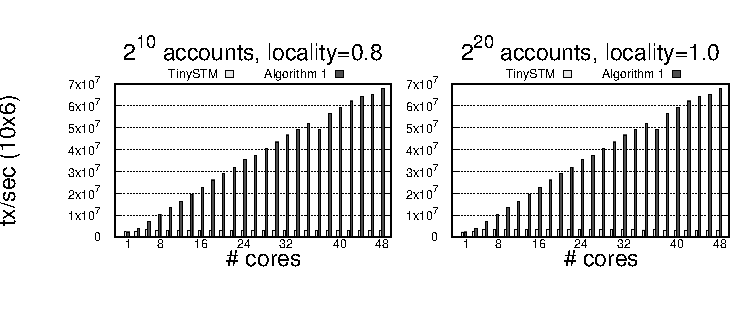
\includegraphics[scale = 1.0]{results/intset/bank.pdf}
	\caption{Bank Benchmark. Left: 80\% locality. Right: 100\% locality.\label{fig:benchmarking:bank}}
\end{figure}

\begin{figure}[!t]
	\centering
	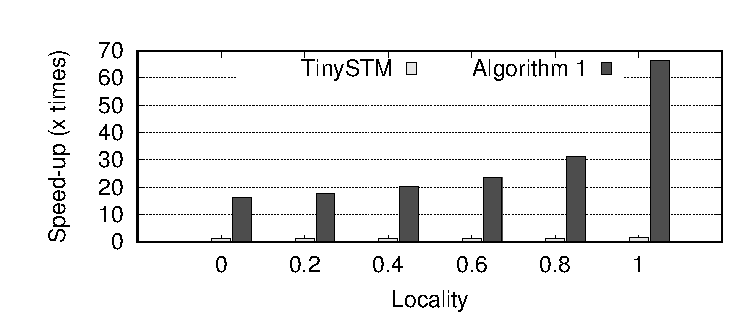
\includegraphics[scale = 0.8]{results/bank-speedup/bank-speedup.pdf}
	\caption{Bank Benchmark. Speed-up of our algorithm for different locality levels. In this experiment, we always use 48 cores.\label{fig:benchmarking:bank:speedup}}
\end{figure}


\subsection{Benchmark: Linked-list}

The linked-list benchmark consists in modifying a sorted linked list concurrently. 
Each thread randomly adds or removes a node from the list. 
We run this benchmark with a range of 512 (meaning that each thread randomly adds/removes a value comprised between -255 and +256) and a linked list initialized with 256 values.
Figure~\ref{fig:benchmarking:llrb}(left) reports our results.

The results show that the global clock outperforms our implementation. 
This is due to the high contention in this application that causes our optimistic algorithm to abort \ft{that's not the right verb} many transactions.

\begin{figure}[!t]
	\centering
	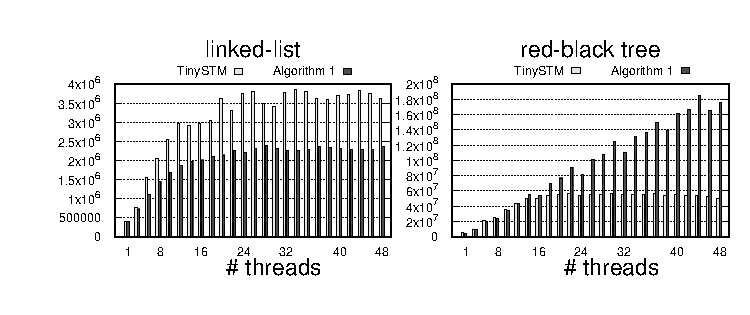
\includegraphics[scale = 1.0]{results/intset/ll-rb.pdf}
	\caption{Linked-list (left) and Red-Black tree (right) benchmarks. Y-axis: transactions/sec. \label{fig:benchmarking:llrb}}
\end{figure}

\subsection{Reb-black tree}

The red-black tree benchmark is similar to the linked-list benchmark except that the values are stored in a self-balancing binary search tree. 
We run this benchmark with a range of $10^7$ values, and a binary tree initialized with $10^5$ values.
Figure~\ref{fig:benchmarking:llrb}(right) reports our results.

When using the global clock, the performance of this application improves linearly up to 12 threads. 
It then stalls to approximately 50 millions transactions per second.

On this application, our implementation scales linearly as the number of threads grows. 
It achieves 176 millions transactions per second with 48 threads.
%
In this benchmark, the likelyhood of a concurrent transaction is very low because of the high number of values in the tree. However,\ft{explain why the global clock performs poorly}.
%

\section{Conclusion}
\labsection{conclusion}

Transactional memory systems must handle a tradeoff between consistency and performance.
It is impractical to take into account all possible combinations of read and write conflicts, as it would lead to largely inefficient solutions.
%% For instance, accepting $\RCAD$ histories brings only a small performance benefits in the general case~\cite{hans16}.

%Inspired by line of research, 
This paper introduces a new consistency criterion, named stricter serializability ($\SPSER$).
Workloads executed under $\SPSER$ are opaque when the object graph forms a tree and transactions traverse it top-down.
We present an algorithm to attain this criterion together with a proof of its correctness.
Our evaluation based on a fully implemented prototype demonstrates that such an approach is very efficient in weakly-contended workloads.

% move from SSER to SSER+ (i.e., alg. transform) ?



%\section{Acknowledgments}

%
% The following two commands are all you need in the
% initial runs of your .tex file to
% produce the bibliography for the citations in your paper.
\bibliographystyle{abbrv}
\bibliography{bib/nicolas,bib/psutra,bib/mshapiro,bib/paper}  % sigproc.bib is the name of the Bibliography in this case
% You must have a proper ".bib" file
%  and remember to run:
% latex bibtex latex latex
% to resolve all references
%
% ACM needs 'a single self-contained file'!
%
%APPENDICES are optional
%\balancecolumns
\end{document}
